% !TEX program = xelatex
%% Requires compilation with XeLaTeX or LuaLaTeX
\documentclass[10pt,xcolor={table,dvipsnames},t]{beamer}
\usepackage{biblatex}
\usepackage{caption}
\setbeamertemplate{caption}[numbered]
\addbibresource{reference.bib}
\usepackage{hyperref}
\hypersetup{ 
pdfpagemode=FullScreen,  
colorlinks=true,linkcolor=blue}
\usepackage{enumerate}
\usepackage{algorithm}
\usepackage{algpseudocode}
\usepackage{listings}
\usepackage{xcolor}

\definecolor{codegreen}{rgb}{0,0.6,0}
\definecolor{codegray}{rgb}{0.5,0.5,0.5}
\definecolor{codepurple}{rgb}{0.58,0,0.82}
\definecolor{backcolour}{rgb}{0.95,0.95,0.92}

\lstdefinestyle{mystyle}{
    backgroundcolor=\color{backcolour},   
    commentstyle=\color{codegreen},
    keywordstyle=\color{magenta},
    numberstyle=\tiny\color{codegray},
    stringstyle=\color{codepurple},
    basicstyle=\ttfamily\footnotesize,
    breakatwhitespace=false,         
    breaklines=true,                 
    captionpos=b,                    
    keepspaces=true,                 
    numbers=left,                    
    numbersep=5pt,                  
    showspaces=false,                
    showstringspaces=false,
    showtabs=false,                  
    tabsize=2
}

\lstset{style=mystyle}

% Flow chart config
\usepackage{tikz}
\usetikzlibrary{calc,trees,positioning,arrows,fit,shapes,calc,tikzmark,matrix}
\usepackage{eso-pic}
\usetikzlibrary{shapes.geometric, arrows}
\tikzstyle{startstop} = [rectangle, rounded corners, minimum width=3cm, minimum height=1cm,text centered, draw=black, fill=red!30]
\tikzstyle{io} = [trapezium, trapezium left angle=70, trapezium right angle=110, minimum width=3cm, minimum height=1cm, text centered, draw=black, fill=blue!30]
\tikzstyle{process} = [rectangle, minimum width=3cm, minimum height=1cm, text centered, draw=black, fill=orange!30]
\tikzstyle{decision} = [diamond, minimum width=3cm, minimum height=1cm, text centered, draw=black, fill=green!30]
\tikzstyle{arrow} = [thick,->,>=stealth]

\usetheme{UCBerkeley}

\title[Your Short Title]{STMC HKOI Training}
\subtitle{Lesson 9: More problem solving techniques}
\author{Chan Yan Mong}
%\institute{}
\date{\today}

\begin{document}

\begin{frame}
  \titlepage
\end{frame}

% Uncomment these lines for an automatically generated outline.
%\begin{frame}{Outline}
%  \tableofcontents
%\end{frame}

\section{Class Goal}

\begin{frame}{Goal today}
\begin{itemize}
  \item Greedy algorithms
  \begin{itemize}
    \item Egyptian Fraction
    \item Best rates 
    \item Changes (Coins problem)
    \item Huffman Code (?)
    \item Interval sceduling
    \item %\href{https://cse.hkust.edu.hk/mjg_lib/Classes/COMP3711H_Fall16/lectures/09greedy.pdf}
  \end{itemize}
  \item Dynamic Programming
  \begin{itemize}
    \item  Knapsack Problem
    \item Number of ways to get from A to B
  \end{itemize}
  \item BFS and DFS
  \begin{itemize}
    \item Potential Map 
    \item Floodfill
    \item Nim game
  \end{itemize}
\end{itemize}

\end{frame}


\begin{frame}[fragile]{Greedy Algorithm}
  \begin{itemize}
    \item \textbf{Greedy algorithm} refers to any algorithm that tries to find/approximate the optimal solution of a problem by making \textit{locally optimal choice} at each stage 
    \item In other words, to find the optimal solution, the algorithm tries to be "greedy", gaining whatever advantage it can gain locally and hope it will converge to something global
    \item Let's look at some examples
  \end{itemize}
\end{frame}

\begin{frame}{Minimum Number of Coins}
  
\end{frame}

\begin{frame}{Egyptian Fraction}
  
\end{frame}

\begin{frame}{Best Rates}
  
\end{frame}

\begin{frame}{Huffman Code}
  
\end{frame}

\begin{frame}[fragile]
\begin{lstlisting}[language=python]
# Searching for names in contact

contact = ['Billy','Damon','Leon','Mary','Shirley']
searchName = input('Enter a name: ')
inContact = False 
for name in contact:
  if searchName == name:
    inContact = True 
if inContact:
  print(f'{searchName} is in contact')

# Search another one
searchName = input('Enter a name again: ')
inContact = False 
for name in contact:
  if searchName == name:
    inContact = True 
if inContact:
  print(f'{searchName} is in contact')
  \end{lstlisting}
\end{frame}

\begin{frame}[fragile]{Code Reusability}
  \begin{itemize}
    \item As shown in the code, line 13 to 19 is completely identical to the above
    \item It would be great if we can put them into one line like this:
\begin{lstlisting}[language=python]
if haveName(contact, name):
  print(f'{name} is in contact')
\end{lstlisting}
    \item \textit{function} provide exactly what we want
  \end{itemize}
\end{frame}

\begin{frame}{Function}
  \begin{columns}
    \begin{column}[T]{0.6\textwidth}
      \begin{itemize}
        \item \textbf{Function}, in the simplest term, is a machine that takes in some input $x$ and perform some action on $x$, producing an output $f(x)$
        \item For example, we may define the following functions:
        \begin{itemize}
          \item $f(x) = x^2$
          \item $f(x) = x^x$
          \item $f(x) = \text{Last digit of x in decimal}$
          \item $f(x) = \{x \quad \text{if} \quad x\geq 0, -x \quad \text{if} \quad x < 0\}$
          \item $f(x,y) = xy^2 + x^2 y^4$
        \end{itemize}
      \end{itemize}
    \end{column}
    \begin{column}[T]{0.4\textwidth}
      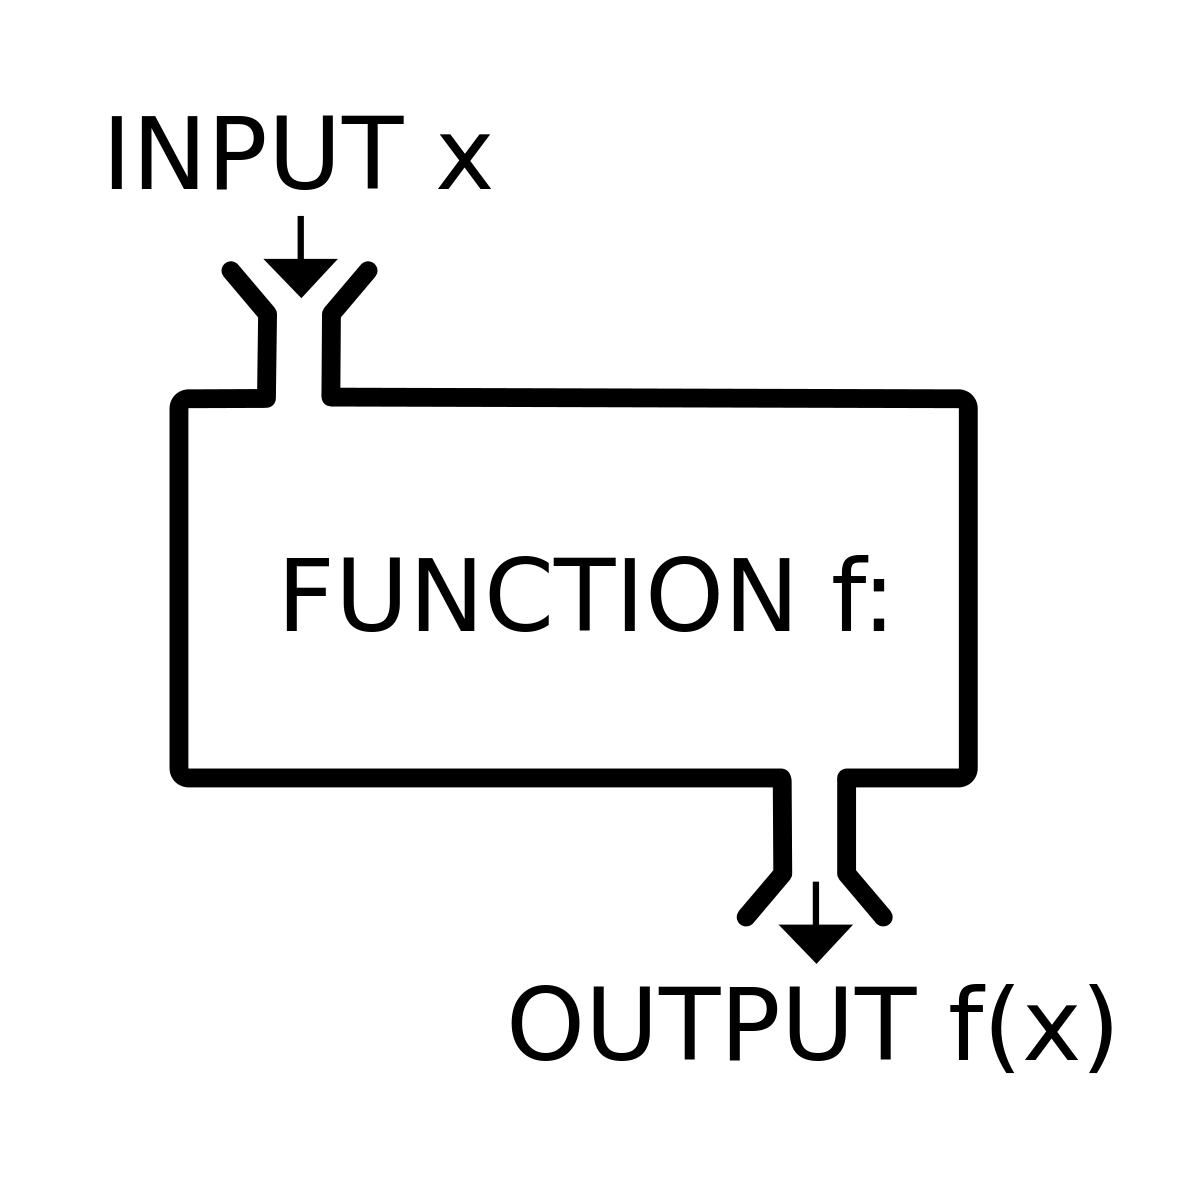
\includegraphics[width=\textwidth]{img/function_as_machine.png}
    \end{column}
  \end{columns}
\end{frame}

\begin{frame}{Function}
  \begin{itemize}
    \item To \textit{evaluate} a function, we put in an input and perform the actions as described by the definition of the $f$. For example:
    \begin{table}[]
      \begin{tabular}{cccc}
                               & \multicolumn{3}{c}{$f(x)$}                                                                            \\ \cline{2-4} 
      \multicolumn{1}{c|}{$x$} & \multicolumn{1}{c|}{$x^2$}    & \multicolumn{1}{c|}{$x^x$}         & $x$ if $x\geq 0$, $-x$ otherwise \\ \hline
      \multicolumn{1}{c|}{-1}  & \multicolumn{1}{c|}{$(-1)^2$} & \multicolumn{1}{c|}{$(-1)^{(-1)}$} & 1                                \\ \cline{1-1}
      \multicolumn{1}{c|}{1}   & \multicolumn{1}{c|}{$(1)^2$}  & \multicolumn{1}{c|}{$(1)^{(1)}$}   & 1                                \\ \cline{1-1}
      \multicolumn{1}{c|}{2}   & \multicolumn{1}{c|}{$(2)^2$}  & \multicolumn{1}{c|}{$(2)^{(2)}$}   & 2                                \\ \cline{1-1}
      \multicolumn{1}{c|}{11}  & \multicolumn{1}{c|}{$(11)^2$} & \multicolumn{1}{c|}{$(11)^{(11)}$} & 11                              
      \end{tabular}
      \end{table}
  \end{itemize}
\end{frame}

\begin{frame}{Function}
  \begin{itemize}
    \item By defining functions, we can simply expressions by "calling" them in our expressions 
    \item For example, $\text{lerp}(a,b,t) = a(1-t) + bt \quad 0\leq t \leq 1$ performs a linear interpolation from $a$ to $b$
    \item By nesting $\text{lerp}$ we can perfrom complicated interpolation
    \begin{align*}
      f(a,b,c,t) = \text{lerp}(\text{lerp}(a,b,t),\text{lerp}(b,c,t),t) 
    \end{align*}
  \end{itemize}
\end{frame}

\begin{frame}{Functions in programming}
  \begin{itemize}
    \item In programming, functions are "self contained" modules of code that accomplish a specific task.
    \item A function takes in certain inputs called the \textbf{arguments} and produce outputs called \textbf{return value}
    \item For example, you may write a \texttt{UserLookup} function that takes in the username as argument, and return user info as return value.
  \end{itemize}
\end{frame}

\begin{frame}[fragile]{Function in programming}
  \begin{itemize}
    \item In python, a function have the following syntax
\begin{lstlisting}[language=python]
def func(arg1,arg2,...):
  # Operations
  return val1,val2,...
\end{lstlisting}
  \item For example, the \texttt{lerp} function just now:
\begin{lstlisting}[language=python]
def lerp(a,b,t):
  return (1-t)*a + t*b
\end{lstlisting}
  \end{itemize}
\end{frame}

\begin{frame}{Function Exercises}
  Complete the following exercises
  \begin{enumerate}
    \item Write a function \texttt{Square(x)} that square a number 
    \item Write a function \texttt{IsBigger(x,y)} that compares two number $x$,$y$ and return True if $x>y$
    \item Write a function \texttt{HaveSubstring(str,substr)} that returns True if \texttt{substr} is contained in \texttt{str} and False otherwise 
    \item Write a function \texttt{SumAll(num\_list)} that return the sum of a list of numbers \texttt{num\_list}
    \item Write a function \texttt{MinMax(num\_list)} that returns in maximum and mininum number from the list \texttt{num\_list}
  \end{enumerate}
\end{frame}

\begin{frame}{Application: Tic-Tac-Toe}
  \begin{itemize}
    \item To demonstrate how function can be used to simply code, we will write a \textit{Tic-Tac-Toe} game
    \item In a Tic-Tac-Toe game, people place \texttt{X} and \texttt{O} in turns until a winning position is obtained
    \item Let's be more specific and write down the actual game flow
  \end{itemize}
\end{frame}

\begin{frame}{Application: Tic-Tac-Toe}
  Here is a possible flow of the game:
  \begin{enumerate}
    \item Prepare an empty $3\times 3$ grid. Assume the game starts with \texttt{X}
    \item Each round, a player enter a pair of numbers $(\text{row},\text{col})$ to specify the row and column he or she wants to place the \texttt{X} (or \texttt{O})
    \item If the position $(\text{row},\text{col})$ is occupied, go back to 2 and ask for re-entry; Otherwise continue
    \item Check if ending position is reached. If so declare the winner and end the game; Otherwise continue 
    \item Change the player from \texttt{X} to \texttt{O} (or \texttt{O} to \texttt{X}) and go back to 2
  \end{enumerate}
\end{frame}

\begin{frame}[fragile]
  With that we can lay down the structure of our code:
\begin{lstlisting}[language=python]
def main():
  grid = [[0,0,0],[0,0,0],[0,0,0]] # Empty 3x3 list
  playerNow = 'X'

  while IsEndPosition(grid) == False:
      row, col = int(input('Row: ')), int(input('Col: '))
      if not Grid_InRange(row,col):
          print(f'The position ({row},{col}) is not in range!')
      elif not Grid_IsEmpty(row,col,grid):
          print(f'The position ({row},{col}) is occupied!')
      else:
          grid[row][col] = playerNow
          playerNow = GetNextPlayer(playerNow)
          Print_Grid(grid)

  winner = IsEndPosition(grid)
  if winner == 'Tie':
      print('Tie!')
  else:
      print(f'{winner} is the winner')
  input()
\end{lstlisting}
\end{frame}


\begin{frame}{Application: Tic-Tac-Toe}
  \begin{itemize}
    \item But wait, what are \texttt{IsEndPosition}, \texttt{Grid\_IsEmpty}, \texttt{GetNextPlayer}, \texttt{Print\_Grid} and  \texttt{Grid\_InRange}
    \item They are \textit{functions} to be defined
    \item As one can see, function allow us to break a program into smaller parts that can be implemented individually
    \item This makes the code cleaner and more maintainable
  \end{itemize}
\end{frame}

\begin{frame}[fragile]
For example, we can implement \texttt{Print\_Grid} like this
\begin{lstlisting}[language=python]
def Print_Grid(grid):
  for i in range(3):
      for j in range(3):
          if grid[i][j] != 0:
              print(grid[i][j],end='')
          else:
              print('-',end='')
      print('')
\end{lstlisting}
ans similarly:
\begin{lstlisting}[language=python]
def Grid_IsEmpty(row,col,grid):
  return grid[row][col] == 0

def Grid_InRange(row,col):
  return 0<=row and row <=2 and 0 <= col and col <= 2

def GetNextPlayer(playerNow):
  if playerNow == 'X':
      return 'O'
  else:
      return 'X'
\end{lstlisting}
\end{frame}

\begin{frame}[fragile]
  For the implementation of \texttt{IsEndPosition}, please refer to the code posted online. Here we will look at some core logic. Basically, we want to check if the grid configuration is in any of these ending positions:
  \begin{itemize}
    \item 3 identical \texttt{X} or \texttt{O} along row 
    \item 3 identical \texttt{X} or \texttt{O} along column
    \item 3 identical \texttt{X} or \texttt{O} along diagonal 
    \item All cells are filled but it is not in any of the ending positions above
  \end{itemize}
  The first two can be done in something like this:
\begin{lstlisting}[language=python]
for i in range(3):
  # Check all rows 
  if grid[i][0] == grid[i][1] and grid[i][0] == grid[i][2] and grid[i][0] != 0:
      return grid[i][0]
  # Check all columns
  if grid[0][i] == grid[1][i] and grid[0][i] == grid[2][i] and  grid[0][i] != 0:
      return grid[0][i]
\end{lstlisting}
\end{frame}


\begin{frame}[fragile]
  The third one can be done like this:
\begin{lstlisting}[language=python]
# Check Diagonals
if grid[0][0] == grid[1][1] and grid[0][0] == grid[2][2] and grid[1][1] != 0:
    return grid[1][1]
if grid[0][2] == grid[1][1] and grid[0][2] == grid[2][0] and grid[1][1] != 0:
    return grid[1][1]
\end{lstlisting}
and the last one can be checked by using this code after excluding all the three cases above:
\begin{lstlisting}[language=python]
# Check if all cells filled
isFull = True
for i in range(3):
    for j in range(3):
        if grid[i][j] == 0:
            isFull = False
            break
\end{lstlisting}
\end{frame}

%    \item For example, following our previous example, we can define the \texttt{haveName} function as:
%\begin{lstlisting}[language=python]
%  def haveName(contact,searchName):
%    inContact = False
%    for name in contact:
%      if searchName == name:
%        inContact = True
%    return inContact
%  \end{lstlisting}


\begin{frame}[fragile]{Recursion}
  \begin{columns}
    \begin{column}{0.6\textwidth}
      \begin{itemize}
        \item Function also allow us to easily implement algorithms that involve \textbf{recursion}
        \item That is, solutions that depends on solutions to smaller instances of the same problem
        \item As we will illustrate, recursion sometimes allow us to solve complicated problems in very neat way
      \end{itemize}
    \end{column}
    \begin{column}[T]{0.4\textwidth}
      \begin{figure}
        
        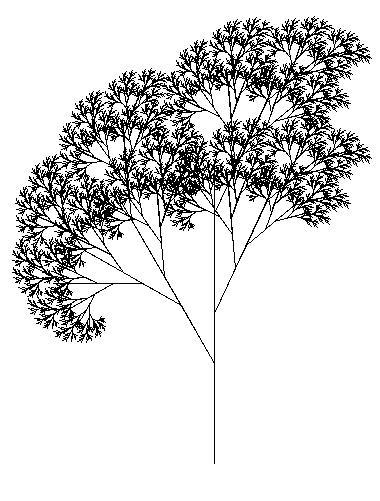
\includegraphics[width=0.7\textwidth]{img/RecursiveTree.JPG}
        \caption{Recursive Tree (\href{https://upload.wikimedia.org/wikipedia/commons/f/f7/RecursiveTree.JPG}{Source})}
      \end{figure}
    \end{column}
  \end{columns}
\end{frame}

\begin{frame}{Example: Fibonacci Sequence}
  \begin{itemize}
    \item Recall the Fibonacci sequence that we discuss long time ago
    \begin{align*}
        &F(n+2) = F(n+1) + F(n)\\
        &F(1) = F(2) = 1
    \end{align*}
    \item We had implemented that using loops before, we will now try to do it in recursion 
  \end{itemize}
\end{frame}

\begin{frame}[fragile]{Example: Fibonacci Sequence}
\begin{lstlisting}[language=python]
# Fibonacci sequence using recursion
  def Fib(n):
  if n == 1 or n == 2:
    return 1
  else:
    return F(n-1) + F(n-2)
\end{lstlisting}
\end{frame}

\begin{frame}{Example: Fibonacci Sequence}
  \begin{itemize}
    \item As shown in the code, calling $F(4)$ returns $F(3)+F(2)$ 
    \item To return $F(3)+F(2)$, we must evaluate $F(3)$ and $F(2)$
    \item $F(2)$ by line 3,4 of the code returns $1$
    \item $F(3)$ on the otherhand calls $F(1)+F(2)$, which both evaluates to $1$ according to line 3,4
    \item So we "backsubstitute" the values layer by layer up and evaluate $F(4) = ((1+1)) + (1) = 3$
  \end{itemize}
\end{frame}

\begin{frame}{Example: Fibonacci Sequence}
  \begin{itemize}
    \item To see what happens for larger $n$, we can consider the following figure
    \begin{figure}
      \centering
      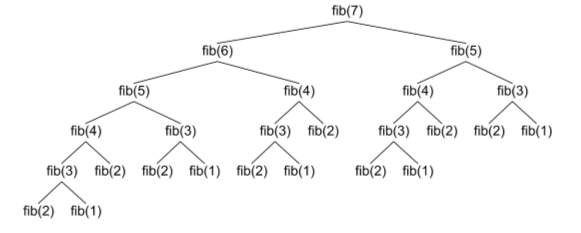
\includegraphics[width=0.8\textwidth]{img/fib-tree.png}      
      \caption*{Source: \href{https://stackoverflow.com/questions/35959100/explanation-on-fibonacci-recursion}{StackOverflow}}
    \end{figure}
  \end{itemize}
\end{frame}

\begin{frame}{Take away}
  This simple exmaple in illustrate some general features of recursive algorithm
  \begin{itemize}
    \item In recursion, we often call a function inside itself (e.g. Here we call $F(3),F(2)$ inside $F(4)$)
    \item Solutions that depends on solutions to
    smaller instances of the same problem (e.g. Finding $F(4)$ involves finding $F(3)$,$F(2)$ )
    \item We combine solutions of smaller problems to solve a larger problem 
  \end{itemize}
\end{frame}


\begin{frame}{Example: Tower of Hanoi}
      \begin{itemize}
        \item The Tower of Hanoi is a mathematical puzzle first introduced by Édouard Lucas in 1883
        \item It begins with the disks stacked on one rod in order of decreasing size, the smallest at the top, thus approximating a conical shape. 
         \item The objective of the puzzle is to move the entire stack to the last rod, obeying the following rules: 
        \begin{enumerate}
          \item Only one disk may be moved at a time.
          \item Each move consists of taking the upper disk from one of the stacks and placing it on top of another stack or on an empty rod.
          \item No disk may be placed on top of a disk that is smaller than it.
        \end{enumerate}
      \end{itemize}
\end{frame}

\begin{frame}{Example: Tower of Hanoi}
  \begin{figure}
    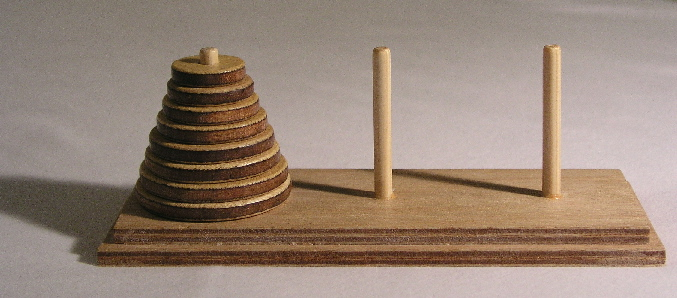
\includegraphics[width=0.8\textwidth]{img/hanoi.jpeg}
  \end{figure}
\end{frame}

\begin{frame}{Example: Tower of Hanoi}
  \begin{itemize}
    \item We would like to program an algorithm that would \textit{solves} the tower of hanoi
    \item Given a stack of $n$ disk to begin with, derive a program that will teach you how should you move the disks to solve the puzzle
    \item Let's try to play around with the game to gain some insights and familiarity
    \item Here is a link to the game: \href{https://www.mathsisfun.com/games/towerofhanoi.html}{https://www.mathsisfun.com/games/towerofhanoi.html}
  \end{itemize}
\end{frame}

\begin{frame}{Example: Tower of Hanoi}
  \begin{exampleblock}{Observations:}
    Suppose there are $n$ disks and suppose we know how to move $n-1$ disks from rod 1 to rod 2. Then to move $n$ disks, we just need to:
    \begin{enumerate}
      \item Move all $n-1$ disk above to the rod in the middle rod
      \item Place the bottom disk to the final rod
      \item Move the $n-1$ disks to the final rod 
    \end{enumerate}
  \end{exampleblock}
\end{frame}

\begin{frame}{Example: Tower of Hanoi}
  \begin{itemize}
    \item In other words, once we know how to move $n-1$ disks, moving $n$ disks is easy
    \item But how do we know how to move $n-1$ disks?
    \item Well, to move $n-1$ disk, we just need to know how to move $n-2$ disks!
    \item Wait how about $n-2$? We don't know how to do that right?
    \item Well, we just have to figure out how to move $n-3$ disks!
    \item $\cdots$
    \item But how to move $2$ disks?
    \item Well, to move $2$ disks, we just need to know how to move $1$ disk
    \item \textbf{But moving 1 disk is trivial!}
  \end{itemize}
\end{frame}

\begin{frame}[fragile]{Example: Tower of Hanoi}
  \begin{itemize}
    \item Now we know how to solve the problem by recursion
  \end{itemize}
\begin{lstlisting}[language=python]
# Solving Tower of Hanoi using recursion 

def Hanoi(n,rod_from,rod_to):
  if n == 1:
    print(f'Move the disk from rod {rod_from} to rod {rod_to}')
  else:
    rod_middle = 6 - rod_from - rod_to
    Hanoi(n-1,rod_from,rod_middle,lv+1)
    print(f'Move the disk from rod {rod_from} to rod {rod_to}')
    Hanoi(n-1,rod_middle,rod_to,lv+1)
\end{lstlisting}
\end{frame}

\begin{frame}{Example: Listing all permutations}
  
\end{frame}



\begin{frame}{Example: Binary Searching}
  
\end{frame}


\begin{frame}{Example: 8 Queen Problem}
  
\end{frame}

\begin{frame}{Example: Sudoku solver}
  

\end{frame}
\end{document}
